\documentclass[aspectratio=169]{beamer}
\usepackage{fontspec}
\usefonttheme{professionalfonts}
\usepackage{amsmath,amssymb,amsthm}
\usepackage{arydshln,mathtools}
\usepackage{bm}
\usepackage{color}
\definecolor{theme}{RGB}{0,73,114}
\usepackage{multicol}
%\usepackage[caption=false]{subfig}
\usepackage{subcaption}
\usepackage{tikz-cd}


\usepackage{comment}

\usepackage{graphicx}
\usepackage{diffcoeff}
\usepackage{dsfont}
\usepackage{mathrsfs}
\usepackage[most]{tcolorbox}

\usepackage{xspace}
\usepackage{appendixnumberbeamer}


\usepackage{media9}
\usepackage[backend=bibtex, style=verbose]{biblatex}

\bibliography{biblio_PH}
%\renewcommand\bibfont{\scriptsize}

\addtobeamertemplate{footnote}{\vspace{-6pt}\advance\hsize-0.5cm}{\vspace{6pt}}
\makeatletter
% Alternative A: footnote rule
\renewcommand*{\footnoterule}{\kern -3pt \hrule \@width 2in \kern 8.6pt}
% Alternative B: no footnote rule
% \renewcommand*{\footnoterule}{\kern 6pt}
\makeatother


\makeatletter
\g@addto@macro\normalsize{%
	\setlength\abovedisplayskip{5pt}
	\setlength\belowdisplayskip{5pt}
	\setlength\abovedisplayshortskip{5pt}
	\setlength\belowdisplayshortskip{5pt}
}
\makeatother

\graphicspath{{./imagesDualField/}}



% Math macros
\DeclareMathOperator*{\grad}{grad}
\DeclareMathOperator*{\Grad}{Grad}
\DeclareMathOperator*{\Div}{Div}
\renewcommand{\div}{\operatorname{div}}
\DeclareMathOperator*{\Hess}{Hess}
\DeclareMathOperator*{\curl}{curl}


\DeclareMathOperator{\tr}{tr}

\DeclareMathOperator{\Dom}{Dom}
\DeclareMathOperator*{\esssup}{ess\,sup}

\newcommand{\bbR}{\mathbb{R}}
\newcommand{\bbI}{\mathbb{I}}
\newcommand{\bbC}{\mathbb{C}}
\newcommand{\bbF}{\mathbb{F}}
\newcommand{\bbA}{\mathbb{A}}
\newcommand{\bbB}{\mathbb{B}}
\newcommand{\bbS}{\mathbb{S}}


\newcommand{\inpr}[3][]{\ensuremath{( #2, \, #3 )_{#1}}}
\newcommand{\dualpr}[3][]{\ensuremath{\langle #2 \, \vert #3 \rangle_{#1}}}

\newcommand{\bilprod}[2]{\langle \langle \, #1, #2 \, \rangle \rangle}
\newcommand*{\dual}[1]{\ensuremath{\widehat{#1}}}


\DeclareMathOperator*{\argmax}{arg\,max}
\DeclareMathOperator*{\argmin}{arg\,min}

\newtheorem{proposition}{Proposition}
\newtheorem{remark}{Remark}
\newtheorem{hypothesis}{Hypothesis}
\newtheorem{assumption}{Assumption}
\newtheorem{conjecture}{Conjecture}


\def\onedot{$\mathsurround0pt\ldotp$}
\def\cddot{% two dots stacked vertically
	\mathbin{\vcenter{\baselineskip.67ex
			\hbox{\onedot}\hbox{\onedot}}%
}}


\setbeamertemplate{blocks}[rounded][shadow]

\setbeamercolor{block body alerted}{bg=alerted text.fg!10}
\setbeamercolor{block title alerted}{bg=alerted text.fg!20}
\setbeamercolor{block body}{bg=structure!10}
\setbeamercolor{block title}{bg=structure!20}
\setbeamercolor{block body example}{bg=green!10}
\setbeamercolor{block title example}{bg=green!20}

% Remove navigation bar
\setbeamertemplate{navigation symbols}{}

\addtobeamertemplate{navigation symbols}{}{%
	\usebeamerfont{footline}%
	\usebeamercolor[fg]{footline}%
	\hspace{1em}%
	\insertframenumber/\inserttotalframenumber
}


\makeatletter \renewcommand\d[1]{\ensuremath{%
		\;\mathrm{d}#1\@ifnextchar\d{\!}{}}}
\makeatother


%% At begin of each section: show current section and all subsections in the section if any
%% At begin of each subsection except first: show only the current section/subsection
\newif\iftocsub
\tocsubtrue
\AtBeginSection[] {
	\begin{frame}[noframenumbering]{Outline}
		\tableofcontents[sectionstyle=show/shaded, subsectionstyle=show/show/hide]
	\end{frame}
	\tocsubfalse
}
\AtBeginSubsection[] {
	\iftocsub
	\begin{frame}[noframenumbering]{Outline}
		\tableofcontents[currentsubsection, sectionstyle=show/shaded, subsectionstyle=show/shaded/hide]
	\end{frame}
	\fi
	\tocsubtrue
}

\newcommand{\beginbackup}{
	\newcounter{framenumbervorappendix}
	\setcounter{framenumbervorappendix}{\value{framenumber}}
}
\newcommand{\backupend}{
	\addtocounter{framenumbervorappendix}{-\value{framenumber}}
	\addtocounter{framenumber}{\value{framenumbervorappendix}} 
}


\begin{document}
	
	
	\begin{frame}[plain]
		
		\input{Title_DualField}
		
	\end{frame}
	
	
	\begin{frame}{Outline}
		
		\tableofcontents
		
	\end{frame}


\section{The geometric structure of port-Hamiltonian systems}

\begin{frame}{A unified language for multiphysics in engineering}
	The port-Hamiltonian (pH) paradigm provides a language to understand multiphysics:
	\vspace{.3cm}

			\begin{itemize}
				\item \textbf{Physics} is at the core: port-Hamiltonian systems are \textbf{passive} with respect to the \textbf{energy storage function}.
				\item The \textbf{topological} and \textbf{metrical} structure of the equation is clearly separated (mimetic discretization).
				\item PH systems are \textbf{closed under interconnection}. 
			\end{itemize}

	\begin{block}{A quest for duality}
		The concept of \textbf{interconnection} and the \textbf{port} behavior of pH systems is mathematically formalized as \textbf{duality pairing}. How exactly is that defined?
	\end{block}
	
	
\end{frame}




\begin{frame}{The geometric structure of pH systems\footcite{courant1990}}
	\begin{definition}[Dirac structure]
		Given a vector space ${F}$ and its dual ${E}=F'$ with respect to the duality product $\dualpr{\cdot}{\cdot} : {E} \times {F} \rightarrow \mathbb{R}$, consider the symmetric bilinear form:
		$$
		\bilprod{({f}_1, {e}_1)}{({f}_2, {e}_2)} := {\dualpr{{e}_1}{{f}_2}} + {\dualpr{{e}_2}{{f}_1}}, \qquad ({f}_i, {e}_i) \in {B} = {F} \times {E}, \; i = 1, 2.
		$$
		A Dirac structure is a linear subspace $\mathcal{D} \subset {B}$ which equals its orthogonal companion with respect to $\left\langle \left\langle \cdot, \cdot \right\rangle \right\rangle$, {\it i.e.} $\mathcal{D} =\mathcal{D}^{[\perp]}$, where:
		$$
		\mathcal{D}^{[\perp]} := \left\{ ({f}, {e}) \in {B} ~ \mid ~ \bilprod{({f}, {e})}{(\widehat{{f}}, \widehat{{e}})} = 0, ~ \forall ~ (\widehat{{f}}, \widehat{{e}}) \in \mathcal{D} \right\}.
		$$
	\end{definition}


\end{frame}



\begin{frame}{Basic of exterior calculus}
Let $\Lambda^k(\Omega)$ is the space of smooth $k$-forms over the Riemannian oriented manifold $\Omega \subset \bbR^n$ with metric $g$ (i.e. the space of smooth sections of the bundle $\mathrm{Alt}^k T^* \Omega$).

\begin{definition}[Wedge product]
The wedge product is the skew-symmetric exterior product of differential forms
\begin{equation*}
	\alpha^k \wedge \beta^l = (-1)^{kl} \beta^l \wedge \alpha^k,
	\qquad \alpha^k \in \Lambda^k(\Omega), \; \beta^l \in \Lambda^l(\Omega).
\end{equation*}
\end{definition}

\begin{definition}[Exterior derivative]
The exterior derivative $\d:\Lambda^k(\Omega) \rightarrow \Lambda^{k+1}(\Omega), \; k\le n-1$ satisfies the following axiomatic properties
\begin{itemize}
	\item $\d f$ for $f \in \Lambda^0(\Omega)$ is the differential of $f$;
	\item $\d{}\d{} f = 0$ for $f \in \Lambda^0(\Omega)$;
	\item Leibniz rule $\d (\alpha^k \wedge \beta^l) = \d\alpha^k \wedge \beta^l + (-1)^k \alpha^k \wedge \d\beta^l$
\end{itemize}
\end{definition}



\end{frame}


\begin{frame}{Basic of exterior calculus}
	
	\begin{definition}[Trace operator]
		The trace operator is defined to be the pull back of the inclusion map $\iota: \partial \Omega \rightarrow \Omega$
		\begin{equation*}
			\tr \omega^k := \iota^*(\omega^k), \qquad \omega^k \in \Lambda^k(\Omega), \quad k\le n-1.  
		\end{equation*}
	\end{definition}

	\begin{definition}[Duality product]
		Forms can be paired on a manifold $M, \; \dim(M)=m$ (e.g. $M=\Omega$ or $M=\partial \Omega$) via
		\begin{equation*}
			\dualpr[M]{\alpha^k}{\beta^{m-k}} := \int_M \alpha^k \wedge \beta^{m-k}, \quad \alpha^{k} \in \Lambda^{k}(M), \quad \beta^{m-k} \in \Lambda^{m-k}(M), \quad k=0, \dots, m.
		\end{equation*}
	
	\end{definition}

	\begin{definition}[Pointwise inner product of forms]\label{eq:local_inpr}
		Let $\alpha^k, \beta^k \in \Lambda^k(\Omega)$. The point-wise inner product is given by
		\begin{equation*}
			\inpr{\alpha^k}{\beta^k} = g^{i_1 j_1} \dots g^{i_k j_k} \alpha_{i_1 \dots i_k} \beta_{j_1 \dots, j_k},
		\end{equation*}
		where $g^{k l} = (\d\xi^k, \d\xi^l)$ are the components of the inverse metric tensor.
	\end{definition}


\end{frame}

\begin{frame}{The Hodge duality}
	
	
	\begin{definition}[Hodge-$\star$ operator]
		The Hodge-$\star$ operator $\star : \Lambda^k(\Omega) \rightarrow \Lambda^{n-k}(\Omega)$ verifies 
		\begin{equation*}
			\alpha^k \wedge \star \beta^k = \inpr{\alpha^k}{\beta^k} \mathrm{vol}, \qquad \alpha^k, \beta^k \in \Lambda^k(\Omega)
		\end{equation*}
		where locally the standard volume form is given by $\mathrm{vol} = \sqrt{|\mathrm{det}(g_{ij})|}\d\xi^1 \wedge \dots \wedge \d\xi^n.$	
\end{definition}

\begin{definition}[$L^2$ inner product]
	\begin{equation*}
		\inpr[\Omega]{\alpha^k}{\beta^k} := \int_\Omega \inpr{\alpha^k}{\beta^k} \mathrm{vol} = \int_\Omega \alpha^k \wedge \star \beta^k, \qquad \alpha, \; \beta \in \Lambda^{k}(\Omega).
	\end{equation*}
\end{definition}

\begin{definition}[Codifferential]
	The codifferential  map $\d{}^{*} : \Lambda^k(\Omega) \xrightarrow{} \Lambda^{k-1}(\Omega)$ is the formal  adjoint of the exterior derivative
	\begin{equation*}
		\inpr[\Omega]{\alpha^k}{\d{}^* \beta^{k+1}} = \inpr[\Omega]{\d \alpha^{k}}{\beta^{k+1}} - \dualpr[\partial \Omega]{\alpha^{k}}{\star \beta^{k+1}}, \qquad \alpha \in \Lambda^k(\Omega), \; \beta \in \Lambda^{k+1}(\Omega).
	\end{equation*}
\end{definition}


\end{frame}



\begin{frame}{Geometric Dirac structure\footcite{vanderSchaft2002}}
	\begin{tcolorbox}[nobeforeafter, colframe=theme,title=Dirac structure for differential forms]%%
	On a Riemannian oriented manifold $\Omega$ consider
	\begin{itemize}
		\item the flows $(f^p_1, \, f^q_2, \, f_\partial^{n-p}) \in F = \Lambda^p(\Omega) \times \Lambda^q(\Omega) \times \Lambda^{n-p}(\partial\Omega)$,
		\item the efforts $(e_1^{n-p}, \, e_2^{n-q}, \, e_\partial^{n-q}) \in E = \Lambda^{n-p}(\Omega) \times \Lambda^{n-q}(\Omega) \times \Lambda^{n-q}(\partial\Omega)$,
	\end{itemize}
	with $p+q=n+1$ and $\Lambda^k(\Omega)$ is the space of smooth $k$-forms. \\
	The following subset $\mathcal{D} \subset F \times E$ defines a Dirac structure
	\begin{equation*}
		\begin{pmatrix}
			{f}^p_1 \\
			{f}^q_2
		\end{pmatrix} = 
		\begin{bmatrix}
				0 & (-1)^{pq+1} \d \\
				\d & 0 \\
		\end{bmatrix}
		\begin{pmatrix}
			{e}^{n-p}_1 \\
			{e}^{n-q}_2
		\end{pmatrix}, \qquad 
		\begin{pmatrix}
			{f}_\partial^{n-p} \\
			{e}_\partial^{n-q}
		\end{pmatrix} = 
		\begin{bmatrix}
			\tr & 0 \\
			0 &  (-1)^p\tr
		\end{bmatrix}
		\begin{pmatrix}
			{e}^{n-p}_1 \\
			{e}^{n-q}_2
		\end{pmatrix}.
	\end{equation*}
The key is that this subset verify the following power balance (Stokes formula)
\begin{equation*}\label{eq:bal_eq}
	\dualpr[\Omega]{e^{n-p}_1}{{f}^p_1} + \dualpr[\Omega]{{e}^{n-q}_2}{f^q_2} + \dualpr[\partial\Omega]{{e}_\partial^{n-q}}{{f}_\partial^{n-p}} = 0.
\end{equation*}
\end{tcolorbox} 

	
\end{frame}

\begin{frame}{Hyperbolic dynamical systems}
	Consider the following dynamical system with boundary input and observation
	\begin{equation*}
	\begin{aligned}
		\begin{pmatrix}
			\partial_t \alpha^p \\
			\partial_t \beta^q\\
		\end{pmatrix} &= 
		-\begin{bmatrix}
			0 & (-1)^{pq+1}\d \\
			\d & 0 \\
		\end{bmatrix}
		\begin{pmatrix}
			\delta_{\alpha} H^{n-p}\\
			\delta_{\beta} H^{n-q}\\
		\end{pmatrix}, \qquad (-1)^p\tr \delta_{\beta} H^{n-q} = u^{n-q}, \\
		y^{n-p} &= \tr \delta_{\alpha} H^{n-p}, 
	\end{aligned}	
	\end{equation*}
where the variational derivative is defined by
\begin{equation*}
	\begin{aligned}
		\left.\diff{}{\varepsilon}\right|_{\varepsilon = 0} H({\mu}^k + \varepsilon \delta {\mu}^k) = \dualpr[\Omega]{\delta_{\mu} H^{n-p}}{\delta {\mu}^k},
	\end{aligned}
\end{equation*}
Considering the following \textbf{port behavior}:
\begin{itemize}
	\item
	the \textbf{storage ports} $$({f}_1^p,\, f_2^q,\, e_1^{n-p}, \, e_2^{n-q}) := (-\partial_t \alpha^p,\,  -\partial_t \beta^q, \,  \delta_{\alpha} H^{n-p}, \,  \delta_{\beta} H^{n-q}),$$
	\item
	the \textbf{interconnection ports} $$({f}_{\partial}^{n-p}, {e}_{\partial}^{n-q}) := ({y}^{n-p}, {u}^{n-q} ).$$
\end{itemize}
Then the dynamical system defines a Dirac structure.

\end{frame}

\begin{frame}{The geometric wave and Maxwell equations}
	Assume $\Omega \subset \bbR^3$. \\
	Case $p=3, \; q=1$ Wave equation. \\
	Hamiltonian $H= \inpr[\Omega]{p^3}{p^3}+ \inpr[\Omega]{\bm{v}^1}{\bm{v}^1}$
	\begin{equation*}
			\begin{aligned}
				\begin{pmatrix}
					\partial_t p^3 \\
					\partial_t \bm{v}^1\\
				\end{pmatrix} &= 
				-\begin{bmatrix}
					0 & \div \\
					\grad & 0 \\
				\end{bmatrix}
				\begin{pmatrix}
					\star p^3\\
					\star \bm{v}^1\\
				\end{pmatrix}, \qquad -\tr \star \bm{v}^1= u^{2}, \\
				y^{0} &= \tr \star p^3.
			\end{aligned}	
	\end{equation*}
	\vspace{.5cm}\\
	Case $p=2, \;q=2$ Maxwell equation.\\
	Hamiltonian $H= \inpr[\Omega]{\bm{D}^2}{\bm{D}^2}+ \inpr[\Omega]{\bm{B}^2}{\bm{B}^2}$
	\begin{equation*}
		\begin{aligned}
			\begin{pmatrix}
				\partial_t \bm{D}^2 \\
				\partial_t \bm{B}^2\\
			\end{pmatrix} &= 
			\begin{bmatrix}
				0 & \curl \\
				-\curl & 0 \\
			\end{bmatrix}
			\begin{pmatrix}
				\star \bm{D}^2 \\
				\star \bm{B}^2 \\
			\end{pmatrix}, \qquad \tr \star \bm{D}^2= u^{1}, \\
			y^{1} &= \tr \star \bm{B}^2. 
		\end{aligned}	
	\end{equation*}
	
\end{frame}

\begin{frame}{What about the functional analytic structure?}
Consider the Sobolev space
\begin{equation*}
	H\Lambda^k(\Omega) := \{\mu^k \in L^2 \Lambda^k(\Omega) \vert \; \d{\mu^k} \in L^2 \Lambda^{k+1}(\Omega)\}, \qquad k=0, \dots, n-1.
\end{equation*}
One could replace spaces of smooth forms with forms living in this Sobolev space. \\
However, the \textbf{Stokes formula} has only been proven when \textbf{more regularity} is present.
\begin{theorem}[D. Arnold \textit{Finite Element Exterior calculus}]
	In a manifold $\Omega$ with Lipschitz boundary it holds
	\begin{equation*}
		\int_\Omega \d{\mu} \wedge \lambda + (-1)^k \int_\Omega \mu \wedge \d{\lambda} = \int_{\partial \Omega}\tr {\mu} \wedge \tr{\lambda}, \qquad \mu \in H^1\Lambda^{k}(\Omega), \quad \lambda \in H \Lambda^{n-k-1}(\Omega),
	\end{equation*}
	where $H^1\Lambda^k(\Omega)$ is the space of $k$-forms with coefficient in $H^1(\Omega)$.
\end{theorem}

Nevertheless, using conforming finite elements for $H\Lambda^k$, one can obtained a discrete version of the power balance (integration by parts).

\end{frame}

\section{Discretization of port-Hamiltonian systems based on Finite Element Exterior calculus}

\begin{frame}{Why the dual field formulation}
	The problem is how to construct a discrete Hodge star
	\begin{equation*}
		\lambda^k = \star \mu^{n-k}, 
	\end{equation*}
	In a finite element context one relies on a weak formulation\footfullcite{hiptmair2001}
	\begin{equation*}
			\inpr[\Omega]{v^k_h}{\lambda^k_h} = (-1)^{k(n-k)}\dualpr[\Omega]{v^k_h}{\mu^{n-k}_h}
	\end{equation*}
	To construct an \textbf{isomorphic Hodge star} \textbf{dual meshes} are needed. Difficulties:
	\begin{itemize}
		\item Constructing high quality dual meshes is difficult and no open software is available;
		\item Mesh entities for the dual mesh lay outside of the physical domain.
	\end{itemize}
	


	If only \textbf{one computational mesh} is used, the weak Hodge corresponds to the \textbf{$L^2$ projection between dual finite element spaces}
	\begin{equation*}
	 \mathbf{M}^k \bm{\lambda}^k =(-1)^{k(n-k)} \mathbf{L}^{n-k} \bm{\mu}^{n-k},
	\end{equation*}
	where $\mathbf{L}^{n-k}$ is rectangular.
\end{frame}


\begin{frame}{How to circumvent the Hodge: the adjoint pH structure}
	Using the \textbf{Hodge isometry} an adjoint pH structure (associated to an adjoint Dirac structure) is computed
	
	\begin{tcolorbox}[nobeforeafter, colframe=theme,title=Adjoint pH system]%%
	\begin{equation*}
		\begin{aligned}
			\begin{pmatrix}
				\partial_t {\alpha}^{n-p} \\
				\partial_t {\beta}^{n-q} \\
			\end{pmatrix} &= -
			\begin{bmatrix}
				0 &  (-1)^{a_0}\d{}^* \\
				(-1)^{a_1}\d{}^* & 0 \\
			\end{bmatrix}
			\begin{pmatrix}
				\delta_{\alpha} \dual{H}^p \\
				\delta_{{\beta}} \dual{H}^q
			\end{pmatrix}, \qquad (-1)^{a_3}\tr \star \delta_{{\beta}} \dual{H}^q= u^{n-q}, \\
			y^{n-p} &= \tr \star \delta_{\alpha} \dual{H}^p,
		\end{aligned}
	\end{equation*}
	where $\d{}^{*}$ is the codifferential and $a_i$ are coefficients due to the Hodge star.
	\end{tcolorbox} 

\end{frame}
	
\begin{frame}{Dual-field discretization\footcite{brugnoli2022df}}
	\begin{itemize}
		\item Combining the port-Hamiltonian system and its adjoint, \textbf{two dynamical systems}, whose dynamics is governed \textbf{by skew-adjoint operators} are constructed.
		\item The two systems are put into \textbf{weak form} considering variables that live in $H\Lambda^k(\Omega)$ using the $L^2$ inner product. The \textbf{codifferential is interpreted weakly} using the integration by parts formula.
		\item \textbf{Conforming finite elements} $\mathcal{V}^k \subset H\Lambda^k(\Omega)$, that give rise to a \textbf{discrete de Rham complex}, are used for the variables.
		\item \textbf{Time integration} performed with \textbf{symplectic Runge-Kutta} method based on Gauss-Legendre collocation points.
	\end{itemize}
	
\end{frame}

\begin{frame}[fragile]\frametitle{The key ingredient for discretization: the De Rham complex}
\centering{
	\begin{tikzcd}
		H\Lambda^0(\Omega) \arrow[r, "\d{}"] \arrow[d, leftrightarrow, "Id"]
		& H\Lambda^{1}(\Omega) \arrow[r, "\d{}"] \arrow[d, "\sharp", xshift=10pt] & H\Lambda^2(\Omega) \arrow[r, "\d{}"] \arrow[d, "\beta^{-1}", xshift=10pt]
		& H\Lambda^{3}(\Omega) \arrow[d, "\star", xshift=10pt]  \\
		H^1(\Omega) \arrow[r, "\grad"] \arrow[d, "\Pi_{s, h}^{-, 0}"]
		& H^{\curl}(\Omega) \arrow[r, "\curl"] \arrow[u, "\flat"] \arrow[d, "\Pi_{s, h}^{-, 1}"] & H^{\div}(\Omega) \arrow[r, "\div"] \arrow[u, "\beta"] \arrow[d, "\Pi_{s, h}^{-, 2}"]
		& L^2(\Omega) \arrow[u, "\star^{-1}"] \arrow[d, "\Pi_{s, h}^{-, 1}"] \\
			\mathrm{CG}_s(\Omega) \arrow[r, "\grad"] 
		& \mathrm{NED}_s^1(\Omega) \arrow[r, "\curl"] & \mathrm{RT}_s(\Omega) \arrow[r, "\div"]
		& \mathrm{DG}_{s-1}(\Omega) 
	\end{tikzcd}  
}

\vspace{1cm}
The finite elements in the figure form a subcomplex of the de Rham complex:
\begin{itemize}
	\item $\grad \mathrm{CG}_s(\Omega) \subset \mathrm{NED}_s^1(\Omega)$,
	\item $\curl \mathrm{NED}_s^1(\Omega) \subset \mathrm{RT}_s(\Omega)$,
	\item $\div \mathrm{RT}_s(\Omega) \subset \mathrm{DG}_{s-1}(\Omega)$.
\end{itemize}	

\end{frame}


\begin{frame}{Illustration: 3D wave equation with mixed boundary conditions}
	Dynamics and constitutive equations:
\begin{equation*}
	\begin{aligned}
		\begin{pmatrix}
			\partial_t p^3 \\
			\partial_t \bm{v}^1\\
		\end{pmatrix} &= 
		-\begin{bmatrix}
			0 & \div \\
			\grad & 0 \\
		\end{bmatrix}
		\begin{pmatrix}
			\delta_{p} H^{0}\\
			\delta_{\bm{v}} H^{2}\\
		\end{pmatrix}, \\
	\end{aligned}	\qquad
\begin{aligned}
	\delta_{p} H^{0} &= \star p^3 := p^0\\
	\delta_{\bm{v}} H^{2} &= \star \bm{v}^1:= \bm{v}^2. \\
\end{aligned}
\end{equation*}
Input-output behavior (the boundary conditions data coincide with the inputs):
\begin{equation*}
	\begin{aligned}
		p^0|_{\Gamma_1} &= u^0_1, \\
	-\bm{v}^2\cdot \bm{n}|_{\Gamma_2}  &= u^{2}_2, \\
	\end{aligned}	\qquad
	\begin{aligned}
		y^2_2 &= -\bm{v}^2\cdot \bm{n}|_{\Gamma_1}, \\
		y^{0}_1 &= p^0|_{\Gamma_2}.
	\end{aligned}
\end{equation*}

\begin{figure}
\centering
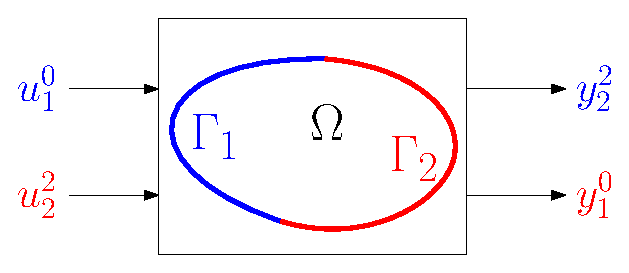
\includegraphics[width=.5\textwidth]{bound_part.eps}
\caption*{Wave equation with mixed \textcolor{blue}{Dirichlet} and \textcolor{red}{Neumann} boundary conditions}
\end{figure}

\end{frame}	

\begin{frame}{The adjoint system}
The initial system
	\begin{equation*}
		\begin{aligned}
			\begin{pmatrix}
				\partial_t p^3 \\
				\partial_t \bm{v}^1\\
			\end{pmatrix} &= 
			-\begin{bmatrix}
				0 & \div \\
				\grad & 0 \\
			\end{bmatrix}
			\begin{pmatrix}
				p^0\\
			 \bm{v}^2\\
			\end{pmatrix}, \\
		\end{aligned}	
	\end{equation*}
The adjoint system

\begin{equation*}
	\begin{aligned}
		\begin{pmatrix}
			\partial_t p^0 \\
			\partial_t \bm{v}^2\\
		\end{pmatrix} &= 
		-\begin{bmatrix}
			0 & \div^* \\
			\grad^* & 0 \\
		\end{bmatrix}
		\begin{pmatrix}
			p^3\\
			\bm{v}^1\\
		\end{pmatrix}, \\
	\end{aligned}	
\end{equation*}

Boundary conditions:
\begin{equation*}
		p^0|_{\Gamma_1} = u^0_1, \qquad
		-\bm{v}^2\cdot \bm{n}|_{\Gamma_2}  = u^{2}_2.
\end{equation*}

\end{frame}

\begin{frame}{Weak formulations}
Introducing Sobolev spaces with boundary conditions	
\begin{equation*}
		H^1_{\Gamma_1}(\Omega) = \{\phi \in H^1(\Omega) |\; \phi|_{\Gamma_1} = 0\}, \qquad
		H^{\div}_{\Gamma_2}(\Omega) = \{\bm{\phi} \in H^{\div}(\Omega) |\; \bm{\phi} \cdot \bm{n}|_{\Gamma_2} = 0\}.
\end{equation*}


\begin{tcolorbox}[nobeforeafter, colframe=theme,title=Primal weak formulation]%%
Find $p^0 \in H^1(\Omega), \; \bm{v}^1 \in H^{\curl}(\Omega)$ such that $p^0|_{\Gamma_1} = u^0_1$ and
\begin{equation*}
	\begin{aligned}
		\inpr[\Omega]{\psi^0}{\partial_t p^0} &= +\inpr[\Omega]{\grad \psi^0}{\bm{v}^1} + \dualpr[\Gamma_2]{\psi^0}{u^2_2}, \\
		\inpr[\Omega]{\bm{\psi}^1}{\partial_t \bm{v}^1} &= -\inpr[\Omega]{\bm{\psi}^1}{\grad {p}^0},
	\end{aligned} \qquad
	\begin{aligned}
		&\forall \psi^0 \in H^1_{\Gamma_1}(\Omega), \\
		&\forall \bm{\psi}^1 \in H^{\curl}(\Omega).
	\end{aligned}
\end{equation*}
\end{tcolorbox} 

\begin{tcolorbox}[nobeforeafter, colframe=theme,title=Dual weak formulation]%%
find $p^3 \in L^2(\Omega), \; \bm{v}^2 \in H^{\div}(\Omega)$ such that $\bm{v}^2 \cdot \bm{n}|_{\Gamma_2} = u^2_2$ and
\begin{equation*}
	\begin{aligned}
		\inpr[\Omega]{\psi^3}{\partial_t p^3} &= -\inpr[\Omega]{\psi^3}{\div\bm{v}^2}, \\
		\inpr[\Omega]{\bm{\psi}^2}{\partial_t \bm{v}^2} &= +\inpr[\Omega]{\div \bm{\psi}^2}{p^3} - \dualpr[\Gamma_1]{\bm{\psi}^2 \cdot \bm{n}}{u^0_1},
	\end{aligned} \qquad
	\begin{aligned}
		&\forall \psi^3 \in L^2(\Omega), \\
		&\forall \bm{\psi}^2 \in H^{\div}_{\Gamma_2}(\Omega).
	\end{aligned}
\end{equation*}
\end{tcolorbox} 
The two formulations are uncoupled.
\end{frame}


\begin{frame}{Discrete formulations}
	\begin{equation*}
		\begin{aligned}
		\mathrm{CG}_{s, \Gamma_1}(\Omega) = \{\phi_h \in \mathrm{CG}_{s}(\Omega) |\; \phi_h|_{\Gamma_1} = 0\}, \\
		\mathrm{RT}_{s, \Gamma_2}(\Omega) = \{\bm{\phi}_h \in \mathrm{RT}_{s}(\Omega) |\; \bm{\phi}_h \cdot \bm{n}|_{\Gamma_2} = 0\}.
		\end{aligned}
	\end{equation*}
	
		
		
		\begin{tcolorbox}[nobeforeafter, colframe=theme,title=Primal weak formulation]%%
		Find $p^0_h \in \mathrm{CG}_{s}(\Omega), \; \bm{v}^1_h \in \mathrm{NED}^1_s(\Omega)$ such that $p^0_h|_{\Gamma_1} = u^0_{1, h}$ and
		\begin{equation*}
			\begin{aligned}
				\inpr[\Omega]{\psi^0_h}{\partial_t p^0_h} &= +\inpr[\Omega]{\grad \psi^0_h}{\bm{v}^1_h} + \dualpr[\Gamma_2]{\psi^0_h}{u^2_{2, h}}, \\
				\inpr[\Omega]{\bm{\psi}^1_h}{\partial_t \bm{v}^1_h} &= -\inpr[\Omega]{\bm{\psi}^1_h}{\grad {p}^0_h},
			\end{aligned} \qquad
			\begin{aligned}
				&\forall \psi^0_h \in \mathrm{CG}_{s, \Gamma_1}(\Omega), \\
				&\forall \bm{\psi}^1_h \in \mathrm{NED}^1_{s}(\Omega).
			\end{aligned}
		\end{equation*}	
			
		\end{tcolorbox} 
	
		
	\begin{tcolorbox}[nobeforeafter, colframe=theme,title=Dual weak formulation]%%
		find $p^3_h \in \mathrm{DG}_{s-1}(\Omega), \; \bm{v}^2_h \in \mathrm{RT}_{s}(\Omega)$ such that $\bm{v}^2_h \cdot \bm{n}|_{\Gamma_2} = u^2_{2, h}$ and
		\begin{equation*}
			\begin{aligned}
				\inpr[\Omega]{\psi^3_h}{\partial_t p^3_h} &= -\inpr[\Omega]{\psi^3_h}{\div\bm{v}^2_h}, \\
				\inpr[\Omega]{\bm{\psi}^2_h}{\partial_t \bm{v}^2_h} &= +\inpr[\Omega]{\div \bm{\psi}^2_h}{{p}^3_h} - \dualpr[\Gamma_1]{\bm{\psi}^2_h \cdot \bm{n}}{u^0_{1, h}},
			\end{aligned} \qquad
			\begin{aligned}
				&\forall \psi^3_h \in \mathrm{DG}_{s-1}(\Omega), \\
				&\forall \bm{\psi}^2_h \in \mathrm{RT}_{s, \Gamma_2}(\Omega).
			\end{aligned}
		\end{equation*}
	\end{tcolorbox} 

	\end{frame}



\begin{frame}{Algebraic realization}	
	\only<1>{
\begin{figure}[tbh]%
	\centering
	\subfloat[][Boundary splitting.]{%
		\label{fig:domain}%
		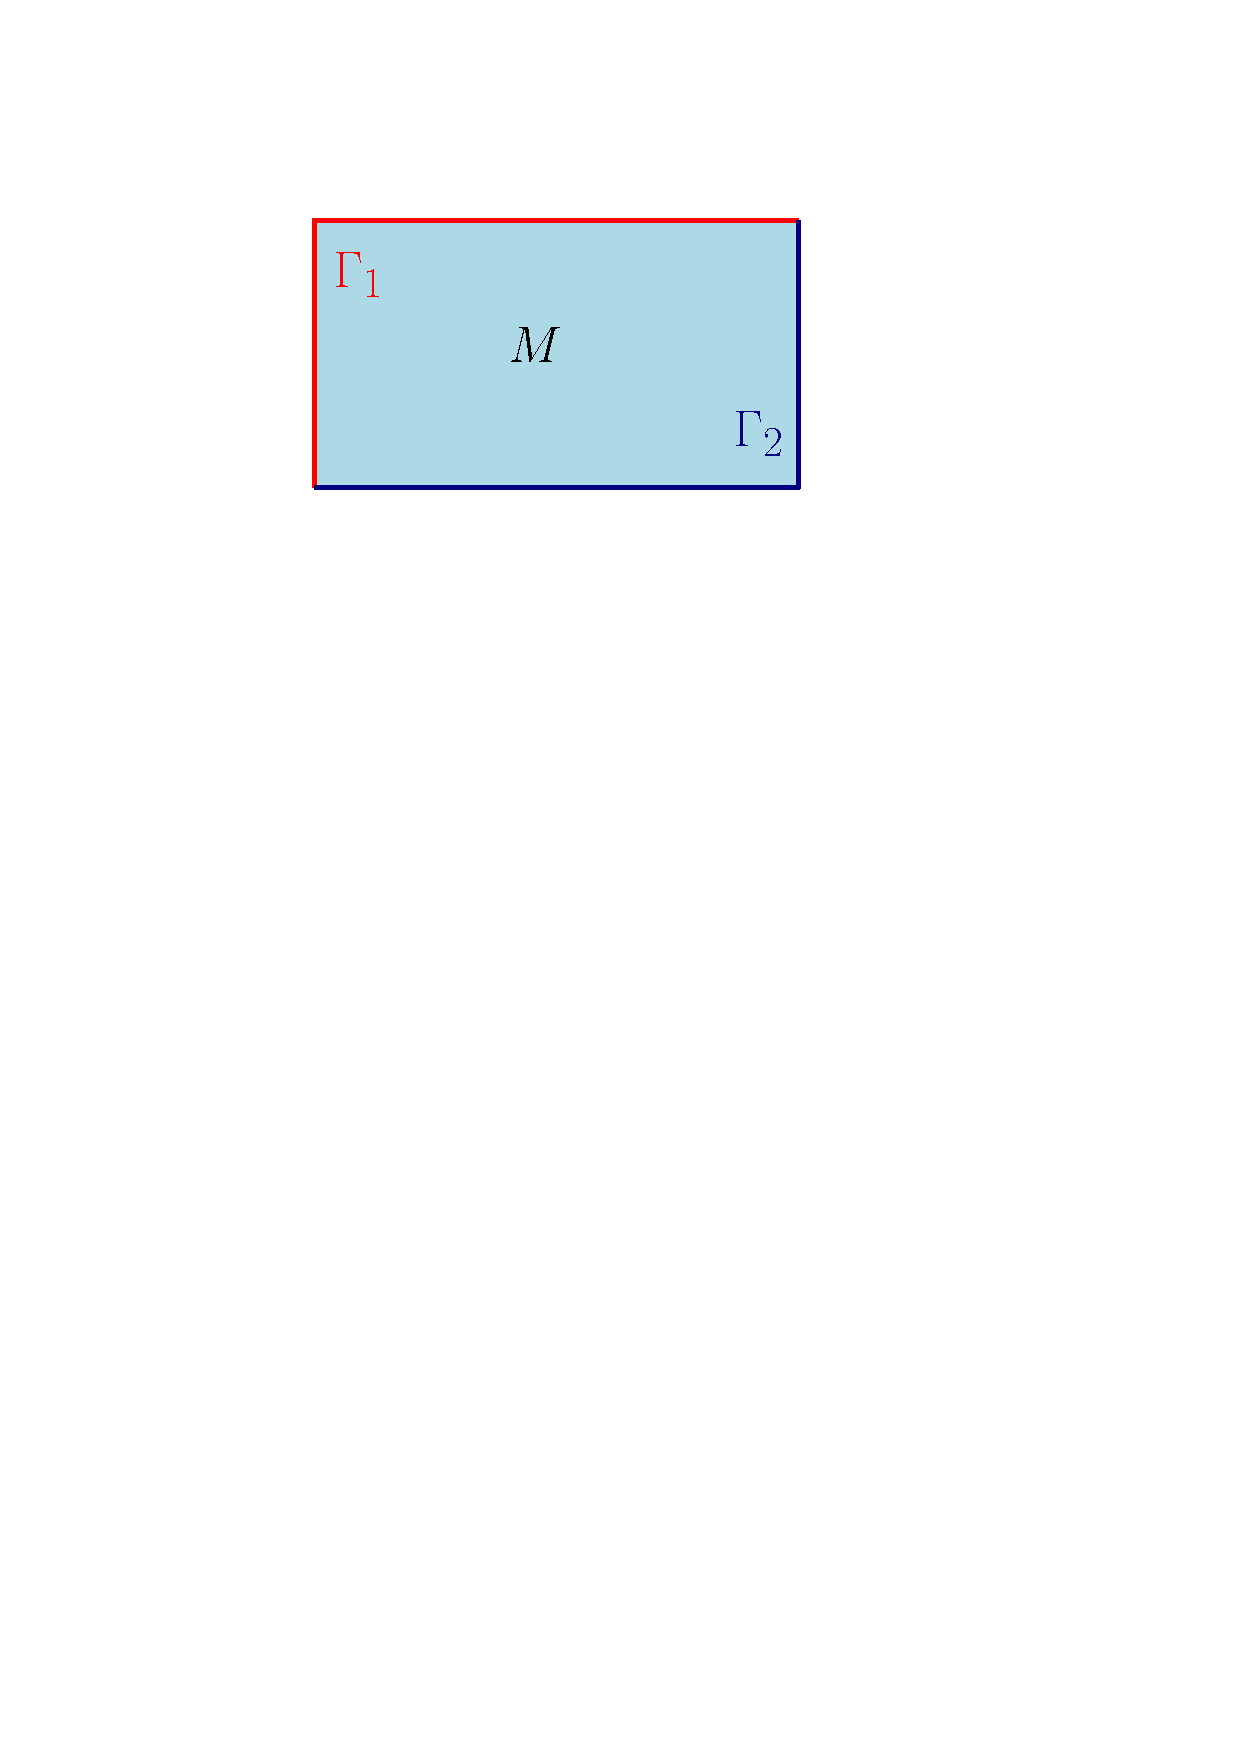
\includegraphics[width=0.4\columnwidth]{domain.pdf}}%
	\hspace{20pt}%
	\subfloat[][Computational mesh]{%
		\label{fig:mesh}%
		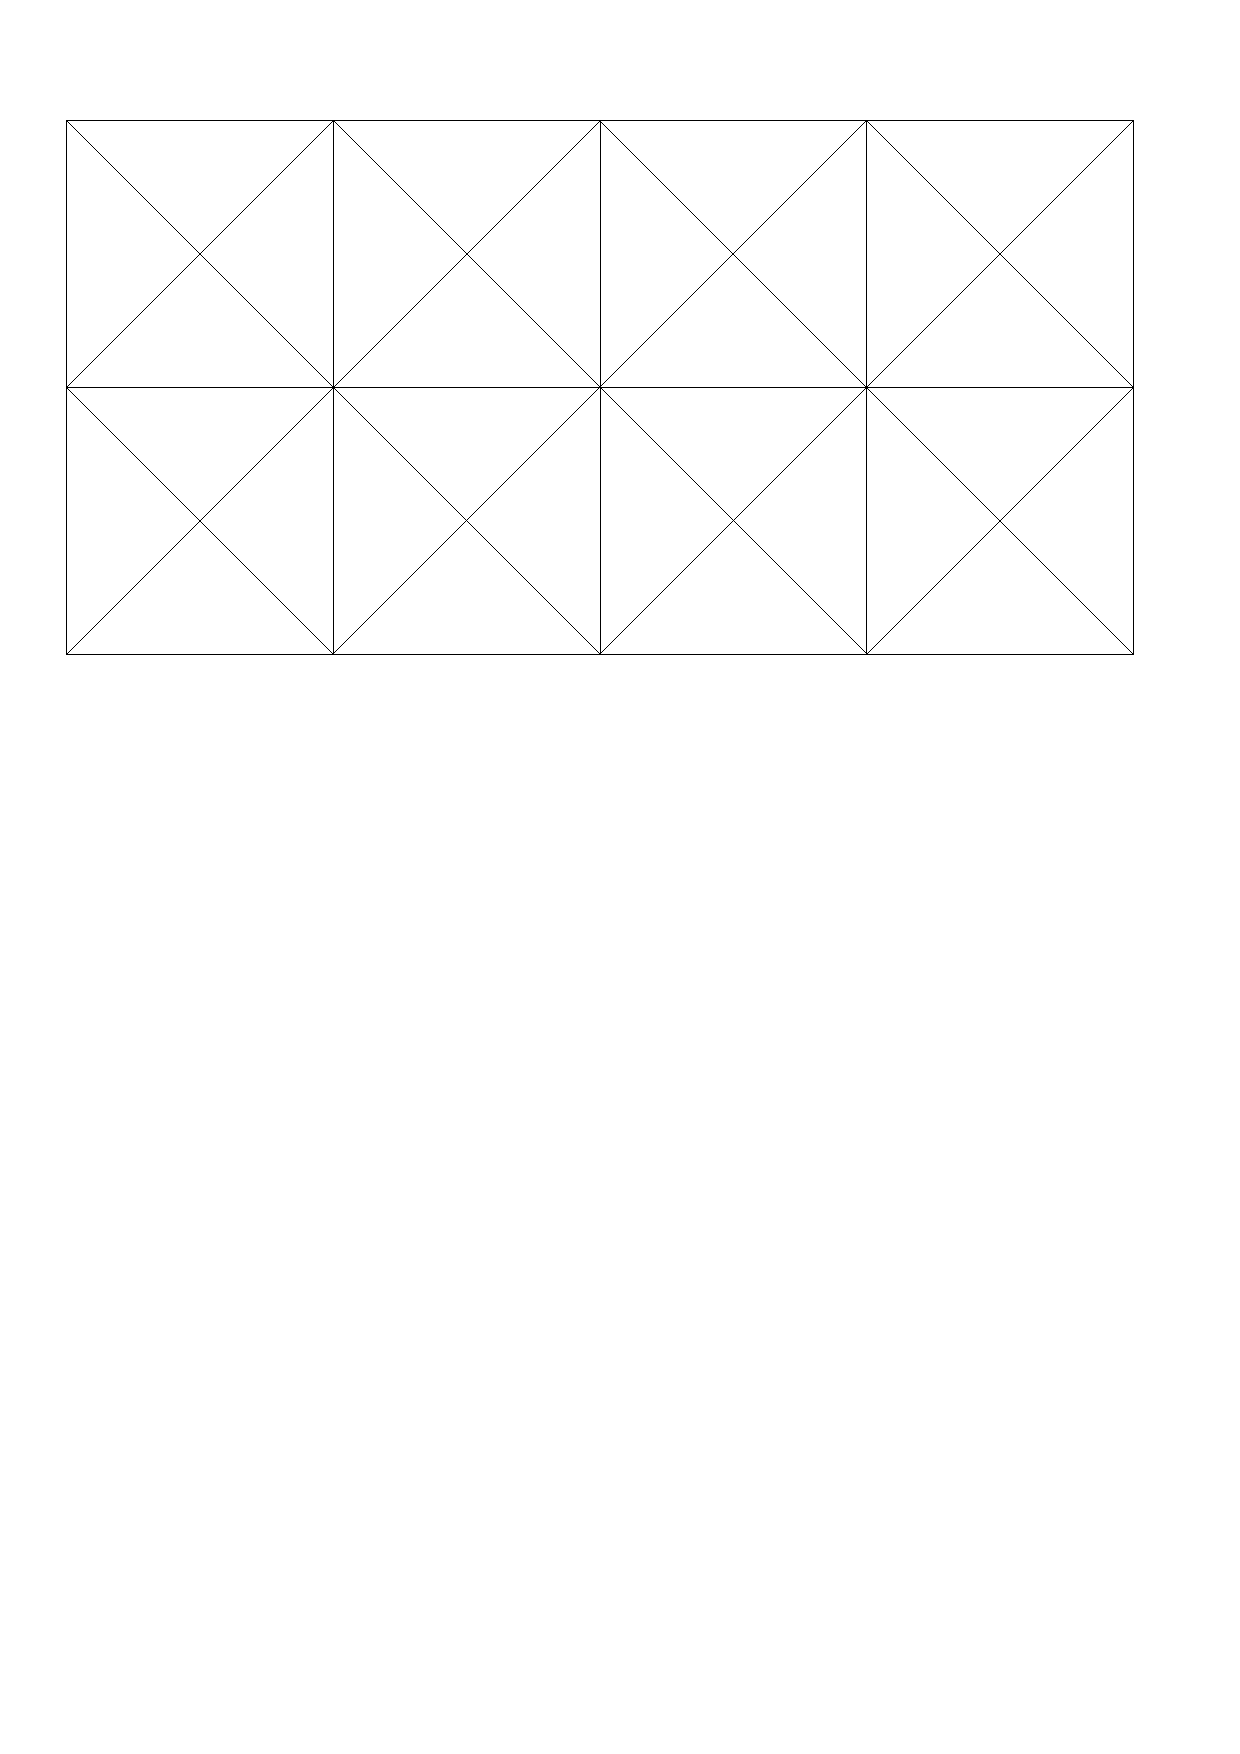
\includegraphics[width=0.4\columnwidth]{mesh.pdf}}%
	\\
	\subfloat[][Dofs 0-form.]{%
		\label{fig:zero_form}%
		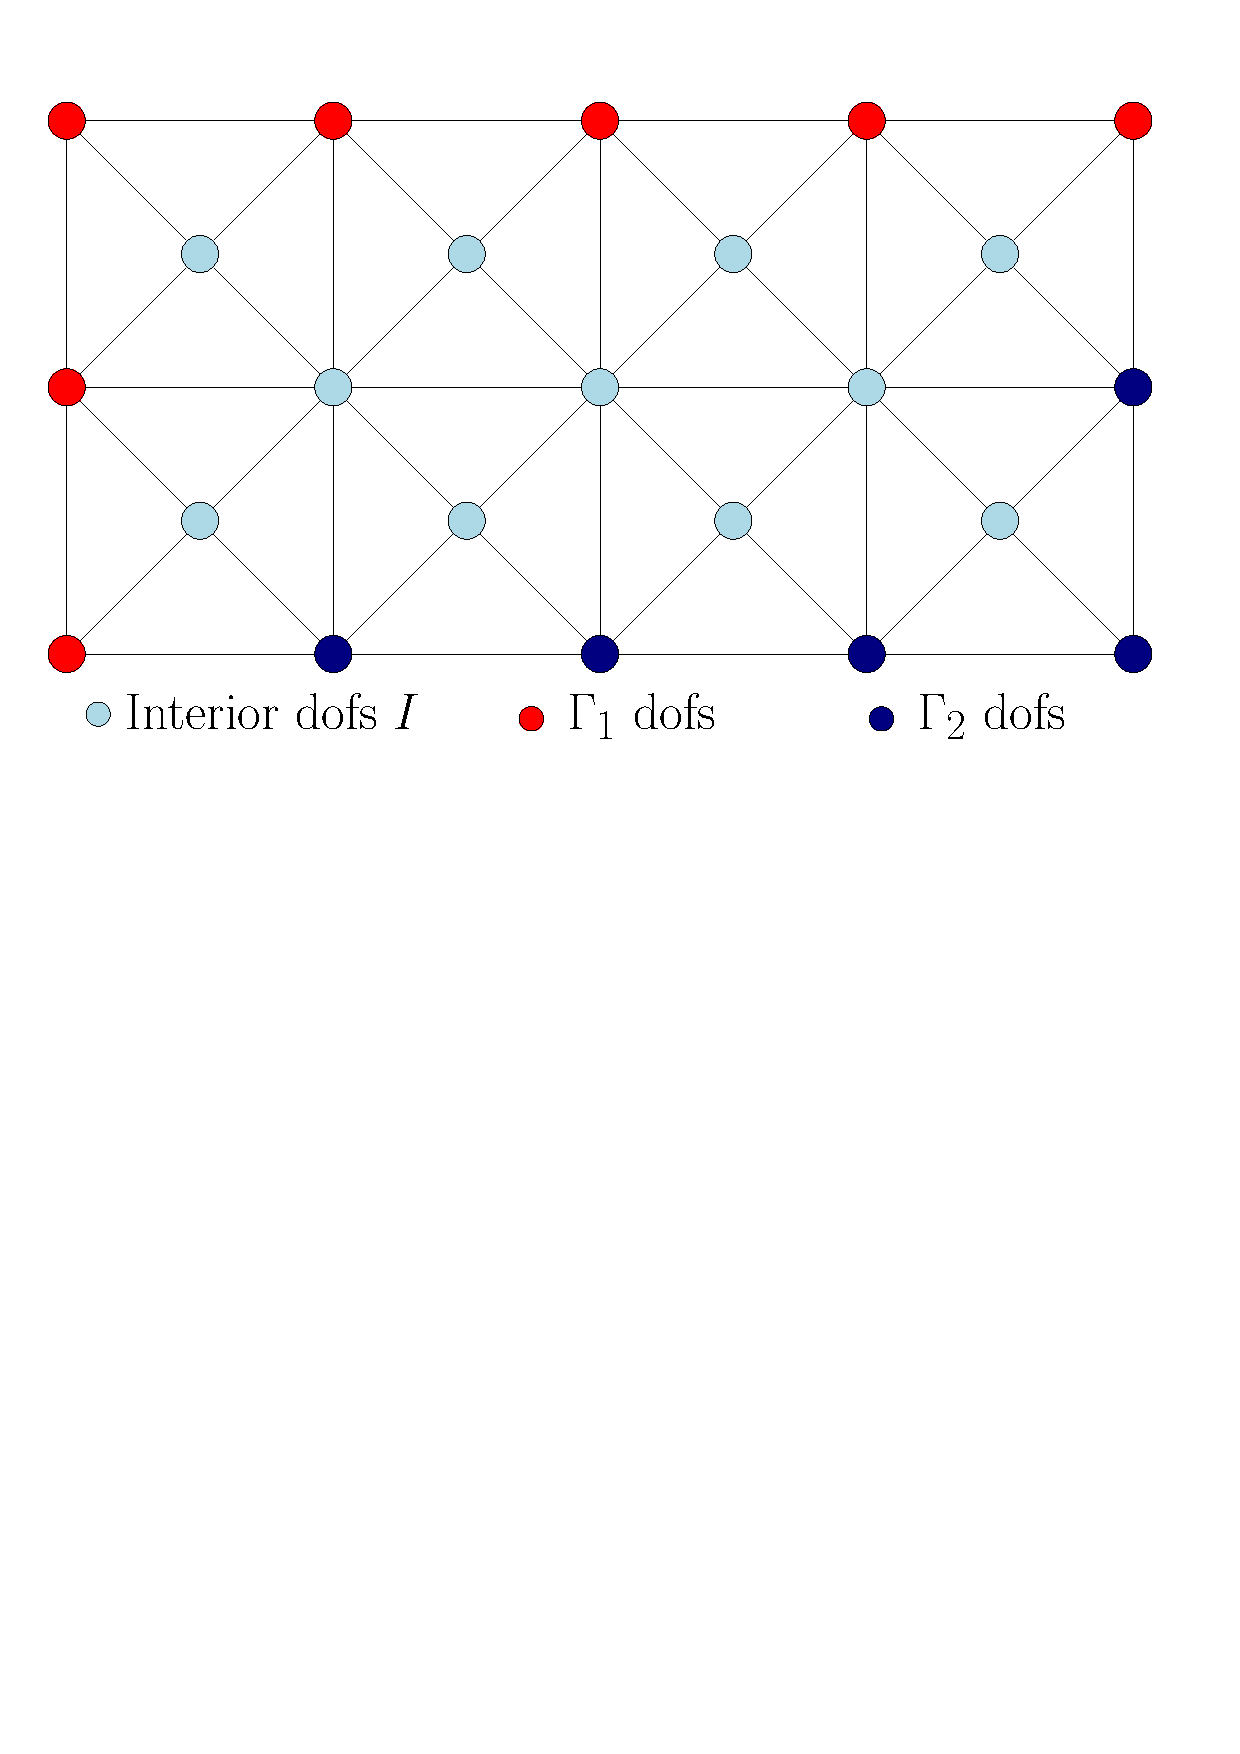
\includegraphics[width=0.4\columnwidth]{zero_form.pdf}}
	\hspace{20pt}%
	\subfloat[][Dofs 1-form.]{%
		\label{fig:one_form}%
		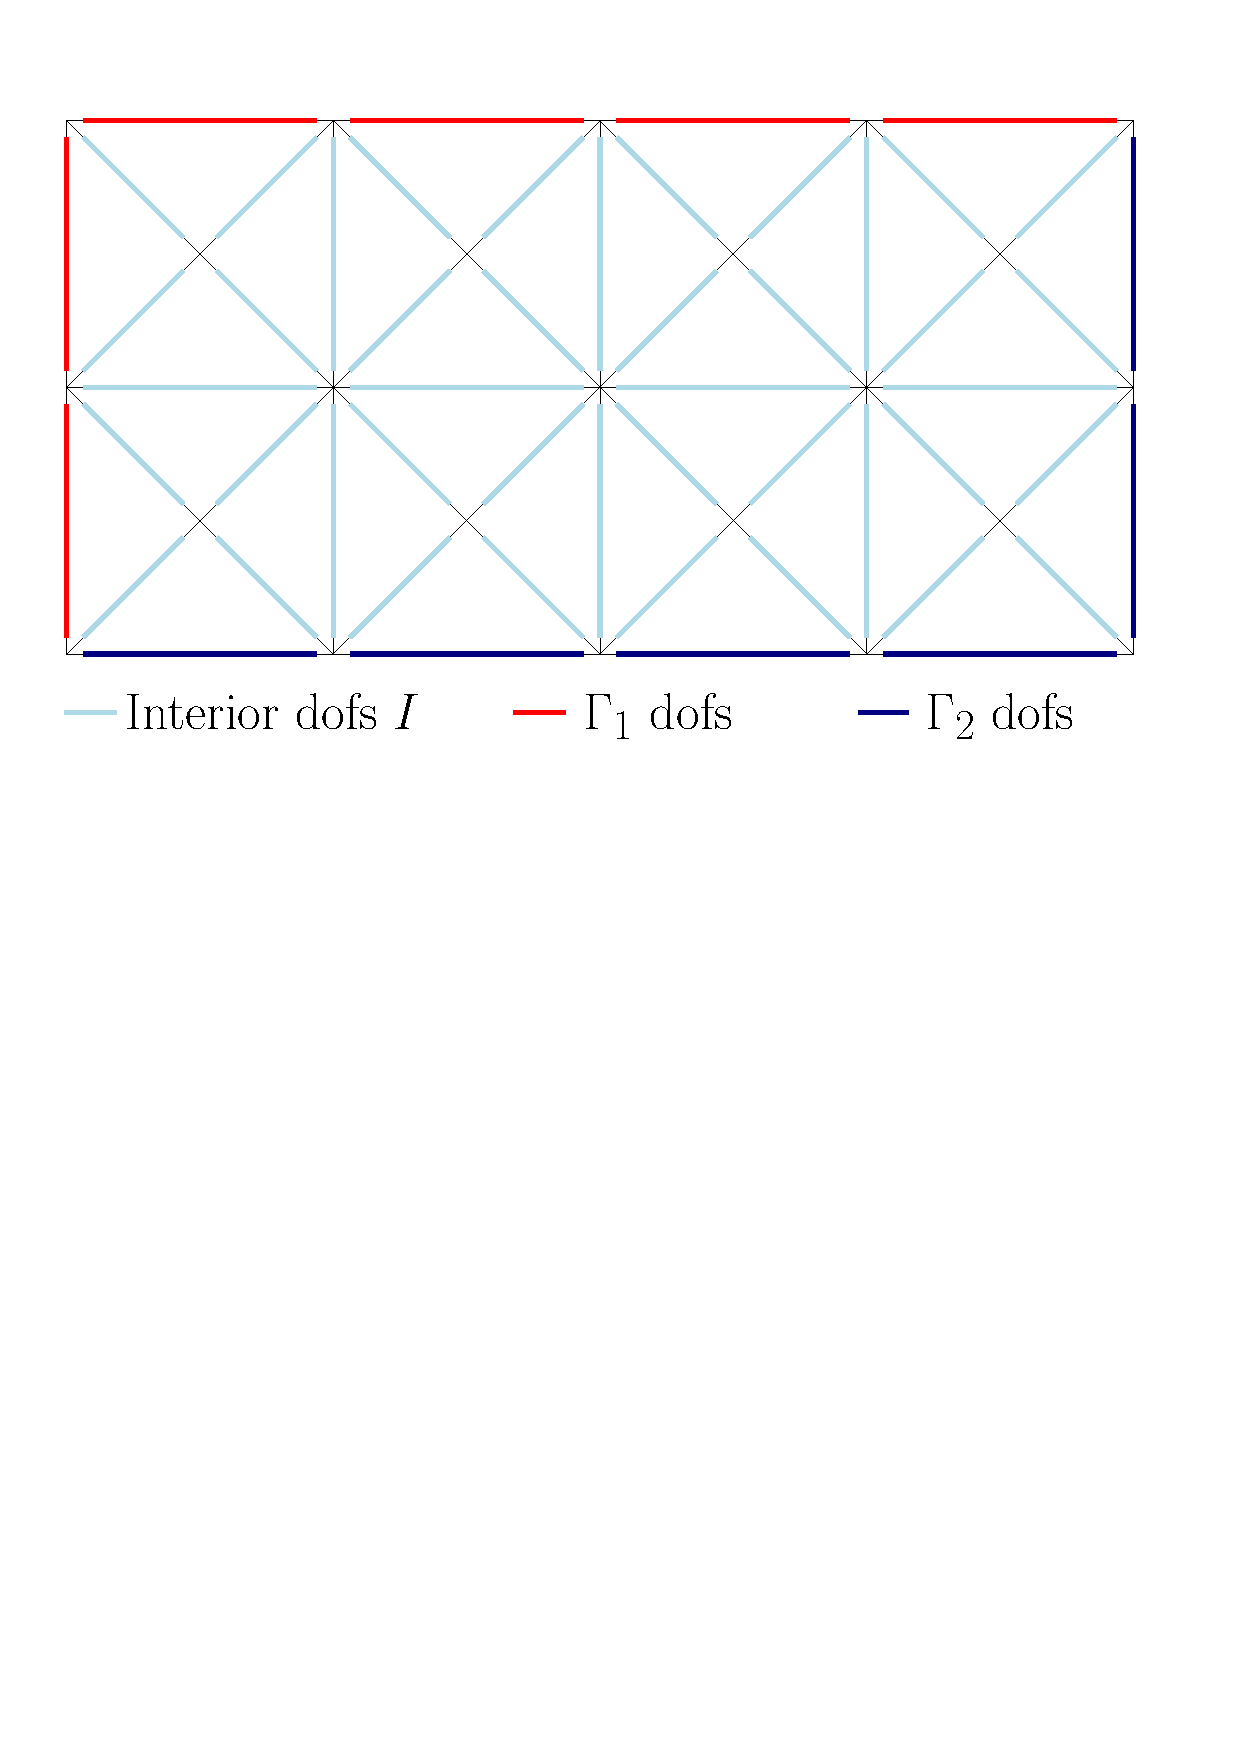
\includegraphics[width=0.4\columnwidth]{one_form.pdf}}
	
\end{figure}	

}
	
	
	\only<2>{
			Given a matrix $\mathbf{A} \in \bbR^{n_R \times n_C}$ the notation $[\mathbf{A}]_{R}^C$ ($R$ and $C$ index sets) indicates the matrix containing the rows and the columns associated with the index set $R$  and $C$.
	\begin{tcolorbox}	
			Algebraic primal formulation
		\begin{equation*}
			\begin{aligned}
				\begin{bmatrix}
					[\mathbf{M}^{0}_{s}]_{I \cup \Gamma_2} & \mathbf{0} \\
					\mathbf{0} & \mathbf{M}^1_{s}
				\end{bmatrix}
				\begin{pmatrix}
					\dot{\mathbf{p}}^{0} \\
					\dot{\mathbf{v}}^1
				\end{pmatrix} &= 
				\begin{bmatrix}
					\mathbf{0} & [(\mathbf{D}_{s}^{0})^\top]_{I \cup \Gamma_2}\\
					-\mathbf{D}^{0}_s & \mathbf{0}
				\end{bmatrix}
				\begin{pmatrix}
					\mathbf{p}^{0} \\
					\mathbf{v}^1
				\end{pmatrix} +
				\begin{bmatrix}
					[\mathbf{B}_{s}^{2}]_{I \cup \Gamma_2}^{\Gamma_2} \\
					\mathbf{0}
				\end{bmatrix}\mathbf{u}^{2}_2, \\
				\mathbf{u}^{0}_1 &= 
				\begin{bmatrix}
					[\mathbf{T}^{0}_{s}]_{\Gamma_1} & \mathbf{0} \\
				\end{bmatrix}
				\begin{pmatrix}
					\mathbf{p}^{0} \\
					\mathbf{v}^1
				\end{pmatrix}
			\end{aligned}
		\end{equation*}
		Algebraic dual formulation
		\begin{equation*}
			\begin{aligned}
				\begin{bmatrix}
					\mathbf{M}^3_{s} & \mathbf{0} \\
					\mathbf{0} & [\mathbf{M}^{2}_{s}]_{I \cup \Gamma_1}
				\end{bmatrix}
				\begin{pmatrix}
					\dot{\mathbf{p}}^3 \\
					\dot{\mathbf{v}}^2 \\
				\end{pmatrix} &=  
				\begin{bmatrix}
					\mathbf{0} & -\mathbf{D}^{2}_s \\
					[(\mathbf{D}_{s}^{2})^\top]_{I \cup \Gamma_1} & \mathbf{0}
				\end{bmatrix}
				\begin{pmatrix}
					{\mathbf{p}}^3 \\
					{\mathbf{v}}^2 \\
				\end{pmatrix} -
				\begin{bmatrix}
					\mathbf{0}\\
					[\mathbf{B}^{0}_{s}]_{I \cup \Gamma_1}^{\Gamma_1}
				\end{bmatrix}
				\mathbf{u}^{0}_1, \\
				{\mathbf{u}}^{2}_2 &= 
				\begin{bmatrix}
					\mathbf{0} & -[\mathbf{T}^{2}_{s}]_{\Gamma_2} \\
				\end{bmatrix}
				\begin{pmatrix}
					{\mathbf{p}}^3 \\
					{\mathbf{v}}^2 \\
				\end{pmatrix}
			\end{aligned}
		\end{equation*}
	\end{tcolorbox} 
}
	
	
\end{frame}



\begin{frame}{Each discretization carries an energy rate}
	Let $[{\Phi}^{0}_{s, \partial}]_{ij} = \dualpr[\partial\Omega]{\bm{\xi}_i^2 \cdot \bm{n}}{\xi^0_j}$ where $\bm{\xi}_i^2, \; \xi^0_j$ are the FE basis at the boundary.
	\begin{proposition}
		The energy rate of the Hamiltonian $H_{\mathrm{primal}} = \frac{1}{2}\{\inpr[\Omega]{p^0_h}{p^0_h} + \inpr[\Omega]{\bm{v}^1_h}{\bm{v}^1_h}\}$ satisfy
		\begin{equation*}
			\diff{{H}_{\mathrm{primal}}}{t} = (\mathbf{u}^{0}_1)^\top \widetilde{\mathbf{y}}^{0} + ({\mathbf{u}}^{2}_2)^\top[{\Phi}^{0}_{s, \partial}]_{\Gamma_2}^{\Gamma_2} \mathbf{y}^{0}_1,
		\end{equation*} 
		where ${\mathbf{y}}^{0}_1 = [\mathbf{p}^{0}]_{\Gamma_2}$ and $
			\widetilde{\mathbf{y}}^{0} := [\mathbf{M}^{0}_{s}]_{\Gamma_1} \dot{\mathbf{p}}^{0} -[(\mathbf{D}_{s}^{0})^\top]_{\Gamma_1} {\mathbf{v}}^1$.
	\end{proposition}

	\begin{proposition}
		The energy rate of the Hamiltonian $H_{\mathrm{dual}} = \frac{1}{2}\{\inpr[\Omega]{p^3_h}{p^3_h} + \inpr[\Omega]{\bm{v}^2_h}{\bm{v}^2_h}\}$ satisfy
	\begin{equation*}
		\diff{{H}_{\mathrm{dual}}}{t} = ({\mathbf{u}}^{2}_2)^\top \widetilde{\mathbf{y}}^{2} + (\mathbf{y}^{2}_2)^\top[{\Phi}^{0}_{s, \partial}]_{\Gamma_1}^{\Gamma_1} \mathbf{u}^{0}_1, 
	\end{equation*} 
	where ${\mathbf{y}}^{2}_2 = -[{\mathbf{v}}^{2}]_{\Gamma_1}$ and $\widetilde{\mathbf{y}}^{2} :=  -[\mathbf{M}^{2}_{s}]_{\Gamma_2} \dot{{\mathbf{v}}}^{2}  +[(\mathbf{D}_{s}^{2})^\top]_{\Gamma_2} {\mathbf{p}}^3$.
	\end{proposition}
\end{frame}

\begin{frame}{Recovery the power balance}
	
	\begin{proposition}[Discrete power balance]
%\vspace*{-\baselineskip}\setlength\belowdisplayshortskip{10pt}
	\begin{equation*}
		\dualpr[\Omega]{p^{0}_h}{\partial_t p^3_h} + \dualpr[\Omega]{\bm{v}^{2}_h}{\partial_t \bm{v}^{1}_h} + \dualpr[\partial \Omega]{\bm{v}^2_h \cdot \bm{n}}{p_{h}^{0}} = 0.
	\end{equation*}
	\end{proposition}
\textbf{Proof} Since the considered FE form a de Rham subcomplex $\div \bm{v}^2_h \subseteq \mathrm{RT}_s$ and $\grad p_h^0 \subseteq \mathrm{NED}_s^1$. Hence by linearity and non degeneracy of the inner product it holds
\begin{equation*}
	\partial_t p_h^3 = -\div \bm{v}^2_h, \qquad \partial_t \bm{v}_h^1 = -\grad p_h^0.
\end{equation*}
	Taking the duality product with $p_h^0$ and $\bm{v}_h^2$ on each cell $T$ of the mesh, summing up and applying Stokes theorem on each cell
\begin{equation*}
	\sum_{T \in \mathcal{T}_h} \dualpr[T]{p_h^0}{\partial_t p_h^3} + \dualpr[T]{\bm{v}^{2}_h}{\partial_t \bm{v}^{1}_h} = -\sum_{T \in \mathcal{T}_h} \dualpr[\partial T]{\bm{v}^2_h \cdot \bm{n}}{p_h^0}
\end{equation*}

From the finite elements properties, $p_h^0$ is continuous across cells as well as the normal component of $\bm{v}^{2}_h$. Therefore, the inter-cell terms vanish, leading to
\begin{equation*}
	\dualpr[\Omega]{p_h^0}{\partial_t p_h^3} + \dualpr[\Omega]{\bm{v}^{2}_h}{\partial_t \bm{v}^{1}_h}  = - \dualpr[\partial \Omega]{\bm{v}^2_h \cdot \bm{n}}{p_h^0}
\end{equation*}

\end{frame}


\begin{frame}{Propagation of an eigensolution in a cavity}
	Box-shaped three-dimensional domain:
	$$\Omega = \{ (x,y,z) \in [0, 1]\times[0, 1/2]\times[0, 1/2] \}.$$ 
	Boundary sub-partitions:
	\begin{equation*}
		\Gamma_1 = \{(x,y,z) \vert \; x=0 \cup y=0 \cup z=0\}, \qquad \Gamma_2 = \{(x, y, z) \vert \; x=1 \cup y=1/2 \cup z=1/2 \}.
	\end{equation*}

Given the functions
\begin{equation*}
	g(x, y, z) = \cos(x) \sin(y) \sin(z), \qquad f(t) = 2 \sin(\sqrt{3} t) + 3 \cos(\sqrt{3} t),
\end{equation*}
an exact solution  is given by
\begin{equation*}\	\begin{aligned}
		p^3_{\mathrm{ex}} &= \star g \diff{f}{t}, \\    
		\bm{v}^1_{\mathrm{ex}} &= -\d{g} f, 
	\end{aligned} \qquad 
	\begin{aligned}
		p^0_{\mathrm{ex}} &= g \diff{f}{t}, \\
		\bm{v}^2_{\mathrm{ex}} &= -\star \d{g} f,
	\end{aligned}
\end{equation*}
The exact solution provides the appropriate inputs to be fed into the system
\begin{equation*}
	u^0_1 =p^0_{\mathrm{ex}}|_{\Gamma_1}, \qquad u^2_2 =  -\bm{v}^2_{\mathrm{ex}} \cdot \bm{n}\vert_{\Gamma_2}.
	\end{equation*}
\end{frame}


\begin{frame}{Results obtained with a direct solver and implicit midpoint}
	
	\only<1>{
		
		\begin{columns}		
			\begin{column}{.45\textwidth}
				\includemedia[
				addresource=/home/andrea/Videos/CandidatureISAE/Wavep33D.mp4,
				activate=pageopen, 
				deactivate=onclick,
				width=7cm, height=6cm,
				flashvars={
					source=/home/andrea/Videos/CandidatureISAE/Wavep33D.mp4
					&%
					autoPlay=true&%
					loop=true%
				}
				]{}{VPlayer.swf}
				$p^3$
			\end{column}
			\begin{column}{.45\textwidth}
				\includemedia[
				addresource=/home/andrea/Videos/CandidatureISAE/Wavep03D.mp4,
				activate=pageopen, 
				deactivate=onclick,
				width=7cm, height=6cm,
				flashvars={
					source=/home/andrea/Videos/CandidatureISAE/Wavep03D.mp4&%
					autoPlay=true&%
					loop=true%
				}
				]{}{VPlayer.swf}
				$p^0$
			\end{column}
		\end{columns}	
	}
	
	\only<2>{
		
		\begin{columns}		
			\begin{column}{.45\textwidth}
				\includemedia[
				addresource=/home/andrea/Videos/CandidatureISAE/Waveu23D.mp4,
				activate=pageopen, 
				deactivate=onclick,
				width=7cm, height=6cm,
				flashvars={
					source=/home/andrea/Videos/CandidatureISAE/Waveu23D.mp4
					&%
					autoPlay=true&%
					loop=true%
				}
				]{}{VPlayer.swf}
				$|\bm{v}^2|$
			\end{column}
			\begin{column}{.45\textwidth}
				\includemedia[
				addresource=/home/andrea/Videos/CandidatureISAE/Waveu13D.mp4,
				activate=pageopen, 
				deactivate=onclick,
				width=7cm, height=6cm,
				flashvars={
					source=/home/andrea/Videos/CandidatureISAE/Waveu13D.mp4&%
					autoPlay=true&%
					loop=true%
				}
				]{}{VPlayer.swf}
				$|\bm{v}^1|$
			\end{column}
			
		\end{columns}	
	}
	
	\only<3>{	
		\begin{figure}
			\centering
			\subfloat[][$||p^3_h - {p}_{\text{ex}}||_{L^2}$]{%
				\label{fig:err_p3}%
				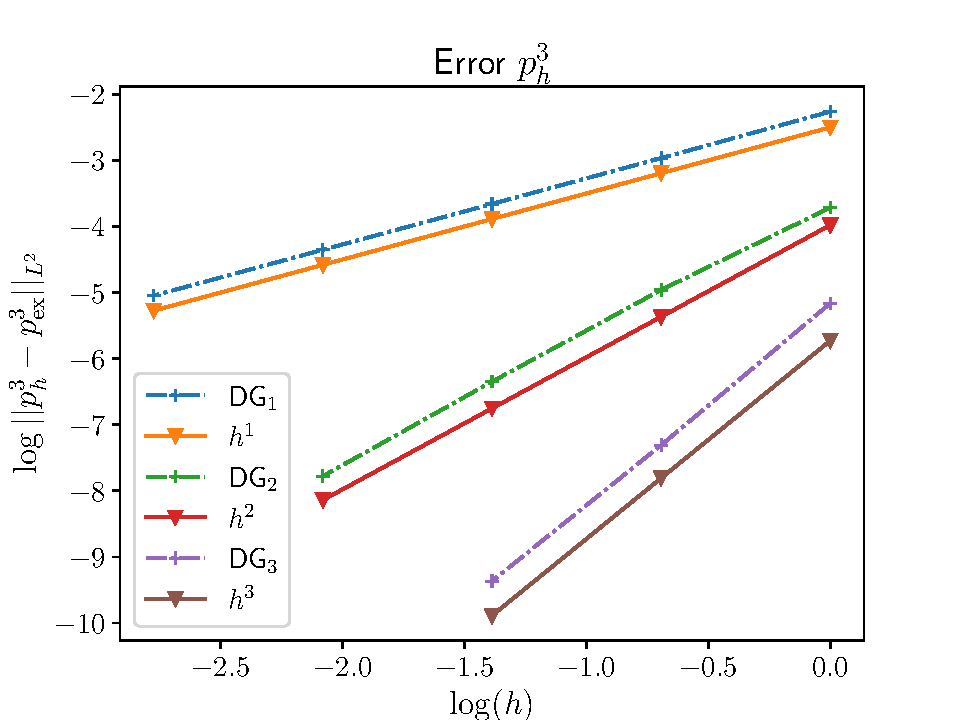
\includegraphics[width=0.48\columnwidth]{p_3_3D_DN.pdf}}%
			\hspace{8pt}%
			\subfloat[][$||p^0_h - {p}_{\text{ex}}||_{L^2}$]{%
				\label{fig:err_p0}%
				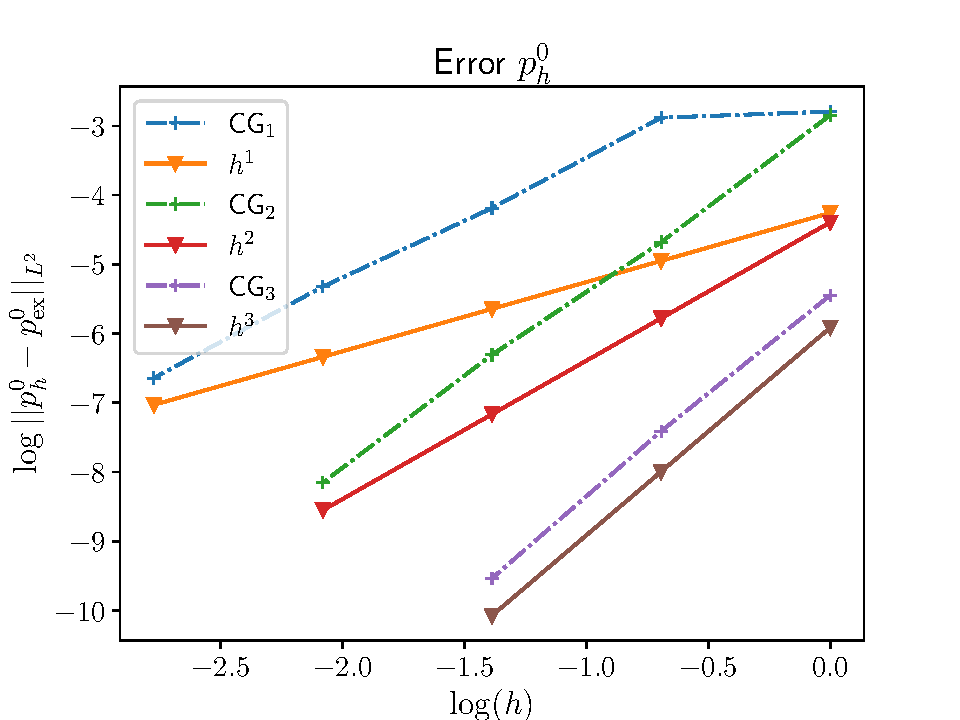
\includegraphics[width=0.48\columnwidth]{p_0_3D_DN.pdf}}%
			\caption*{Convergence rate for $p$}%
		\end{figure}
	}
	\only<4>{	
		\begin{figure}
			\centering
			\subfloat[][$||\bm{v}^1_h - \bm{v}_{\text{ex}}||_{L^2}$]{%
				\label{fig:err_u1}%
				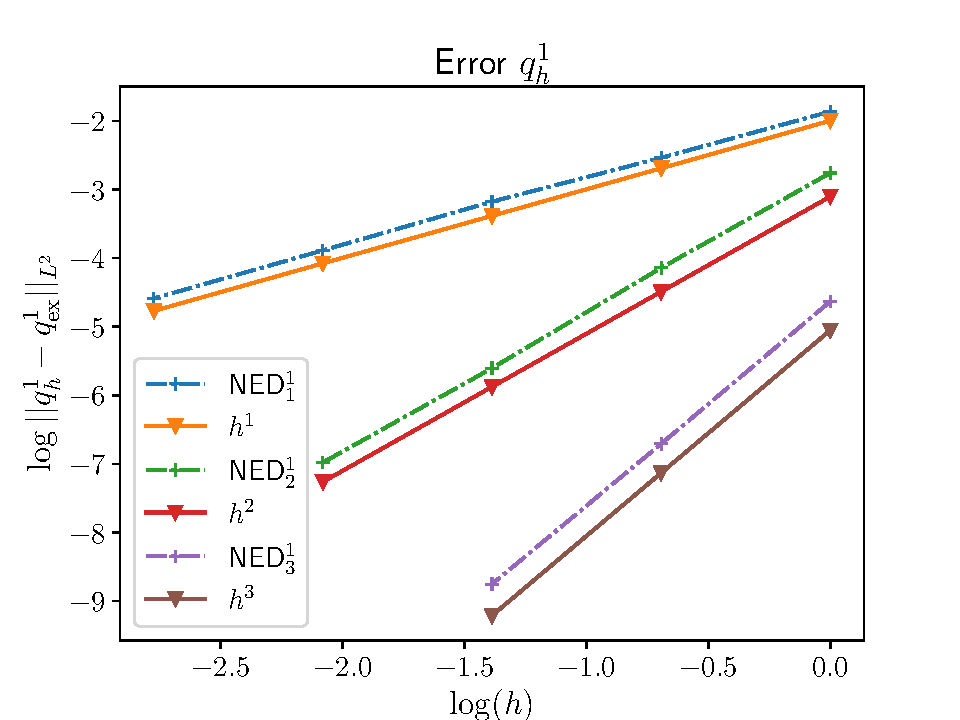
\includegraphics[width=0.48\columnwidth]{q_1_3D_DN.pdf}}
			\hspace{8pt}%
			\subfloat[][$||\bm{v}^2_h - \bm{v}_{\text{ex}}||_{L^2}$]{%
				\label{fig:err_u2}%
				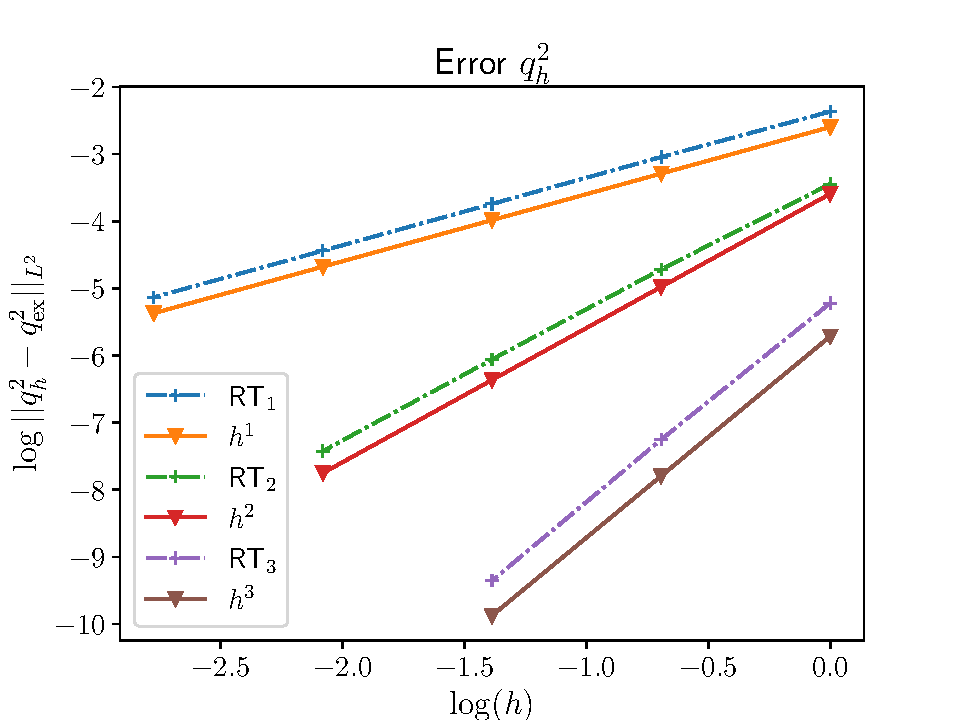
\includegraphics[width=0.48\columnwidth]{q_2_3D_DN.pdf}}
			\caption*{Convergence rate for $\bm{v}$}%
		\end{figure}
	}
	\only<5>{
		\begin{figure}
			\centering
			\subfloat[][$||p^3_h - p^0_h||_{L^2}$]{%
				\label{fig:diff_p30}%
				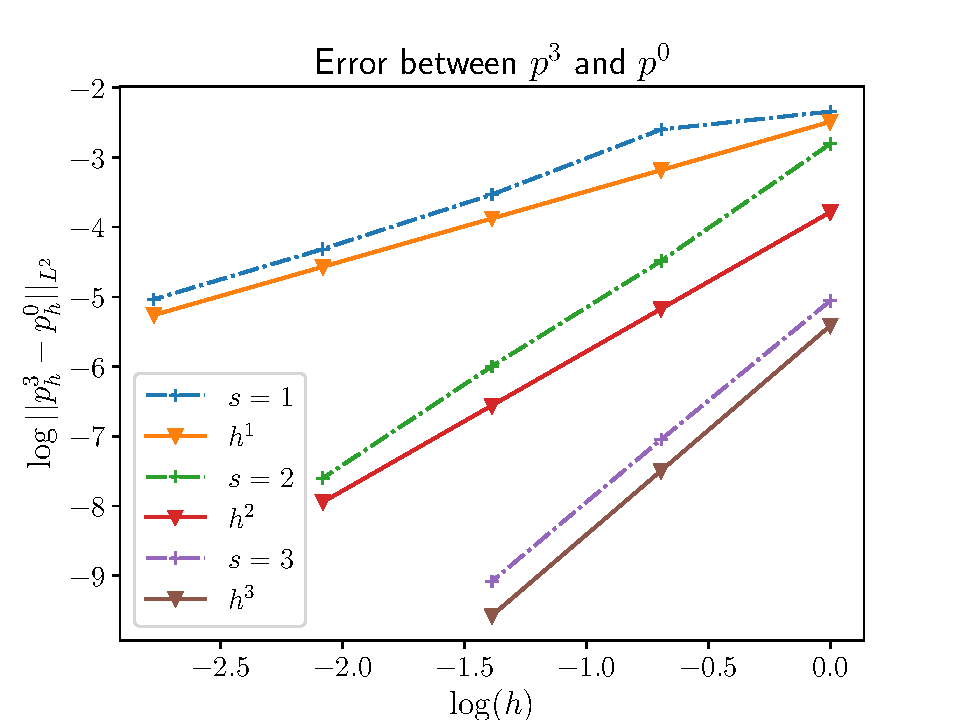
\includegraphics[width=0.48\columnwidth]{p_30_3D_DN.pdf}}%
			\hspace{8pt}%
			\subfloat[][$||\bm{v}^1_h - \bm{v}^2_h||_{L^2}$]{%
				\label{fig:diff_q12}%
				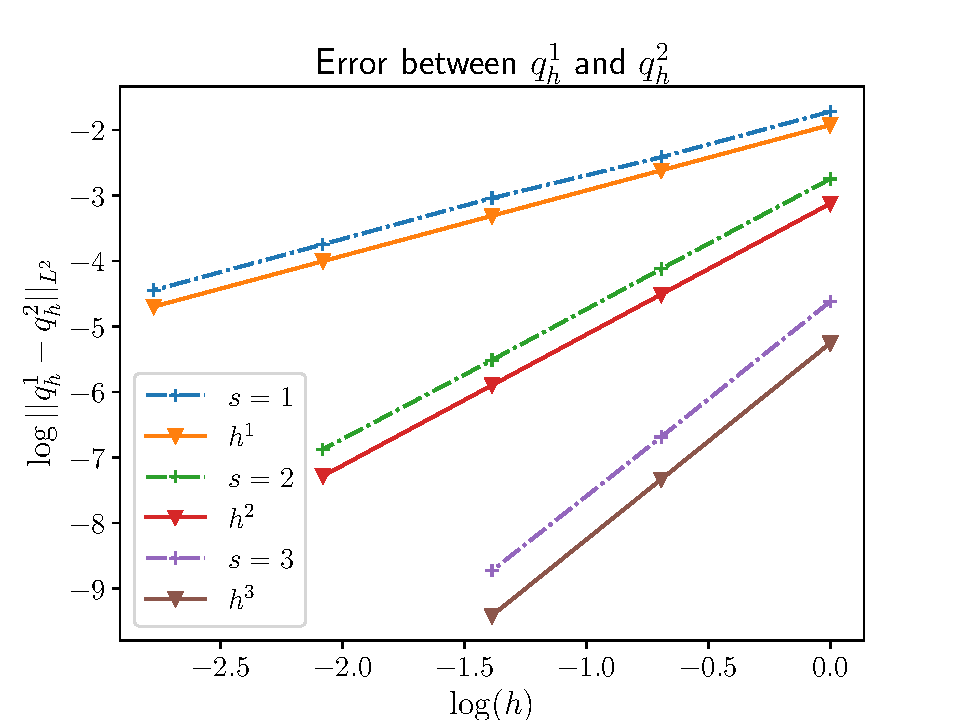
\includegraphics[width=0.48\columnwidth]{q_12_3D_DN.pdf}}%
			\caption*{$L^2$ norm of the difference between dual representation.}%
		\end{figure}
	}

\only<6>{
\begin{figure}[p]%
		\centering
		\subfloat[][Conservation of $P_h-<\dual{e}_{\partial, h}^2|f_{\partial, h}^0>_{\partial M}$]{%
			\label{fig:con_P_wave}%
			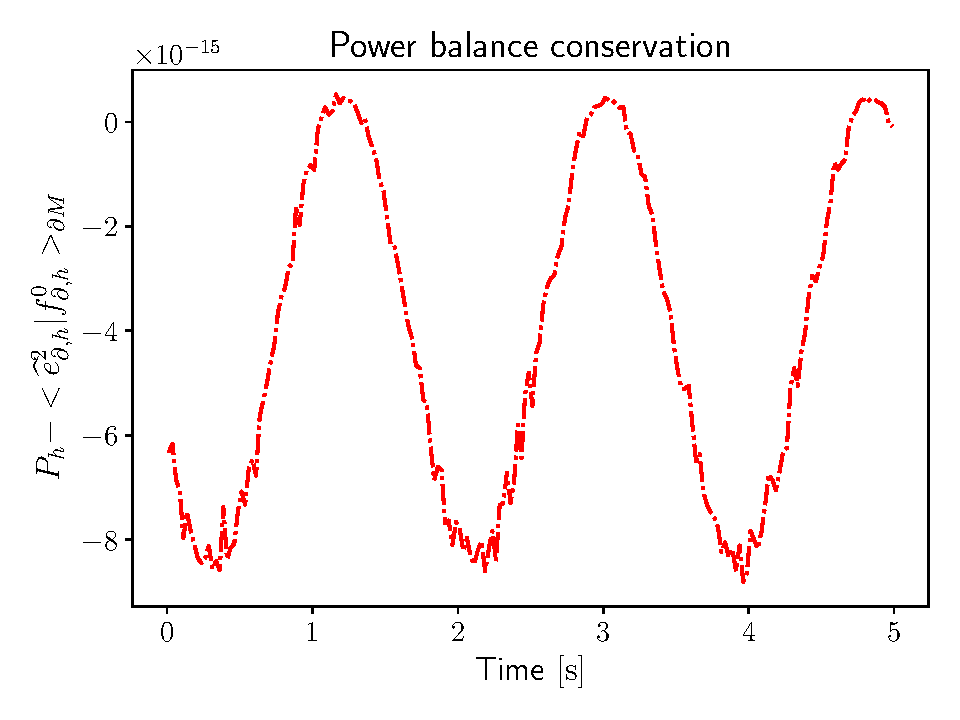
\includegraphics[width=0.48\columnwidth]{pow_bal_3D_DN.pdf}}%
		\subfloat[][Error exact and interpolated boundary flow]{%
			\label{fig:err_flow_wave}%
			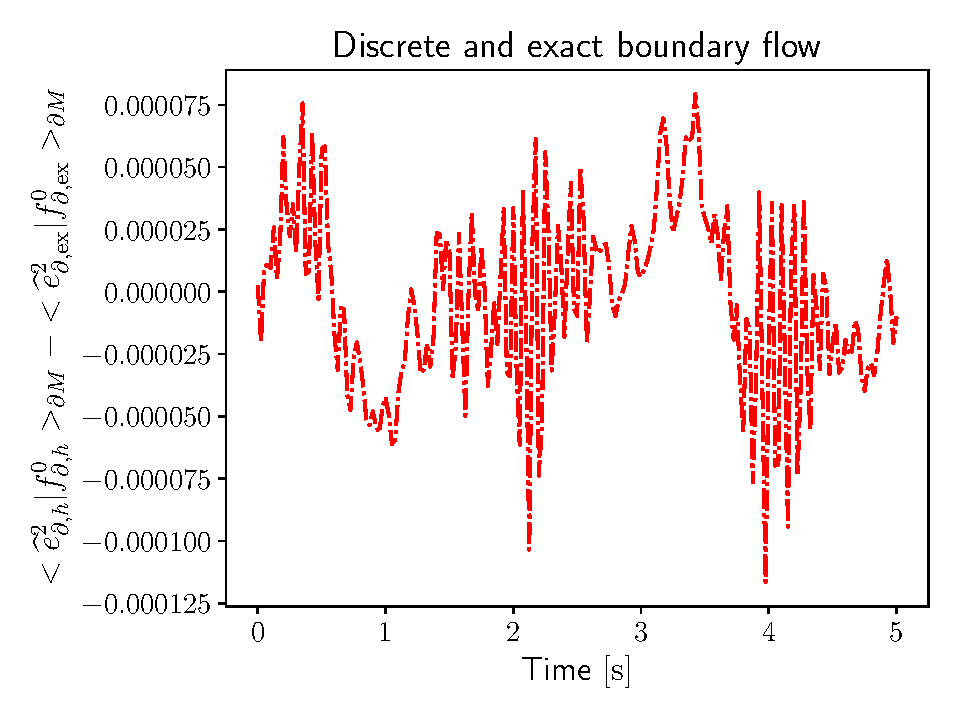
\includegraphics[width=0.48\columnwidth]{bd_flow_3D_DN.pdf}}%
		\caption*{Discrete power balance (left) and error on the power flow (right).}%
		\label{fig:con_pow_wave}%
	\end{figure}
}
	
	
	
\end{frame}

\begin{frame}{Conclusion}
	The open character of pH systems has the \textbf{potential to improve the status quo} of multiphysics simulation.  \\
	\vspace{.3cm}
	\begin{tcolorbox}[nobeforeafter, colframe=theme,title=Analytical developments]%%
	\begin{itemize}
		\item incorporation of geometric and functional analytic aspects;
		\item extension of the geometric theory to continuum mechanics.
	\end{itemize}
	\end{tcolorbox} 
	\vspace{.3cm}\\
	\begin{tcolorbox}[nobeforeafter, colframe=theme,title=Application oriented developments]%%
	\begin{itemize}
		\item efficient algebraic strategies for the resolution of large-scale pH models;
		\item model reduction of models arising from PDEs discretization.
	\end{itemize}
	\end{tcolorbox}

\end{frame}
	
\begin{frame}{Bibliography}
	%\bibliographystyle{unsrt}
	%\nocite{*}
	\printbibliography
\end{frame}

	\appendix
	
	
	
	
\end{document}